% Created by tikzDevice version 0.6.2-92-0ad2792 on 2013-03-06 20:41:48
% !TEX encoding = UTF-8 Unicode
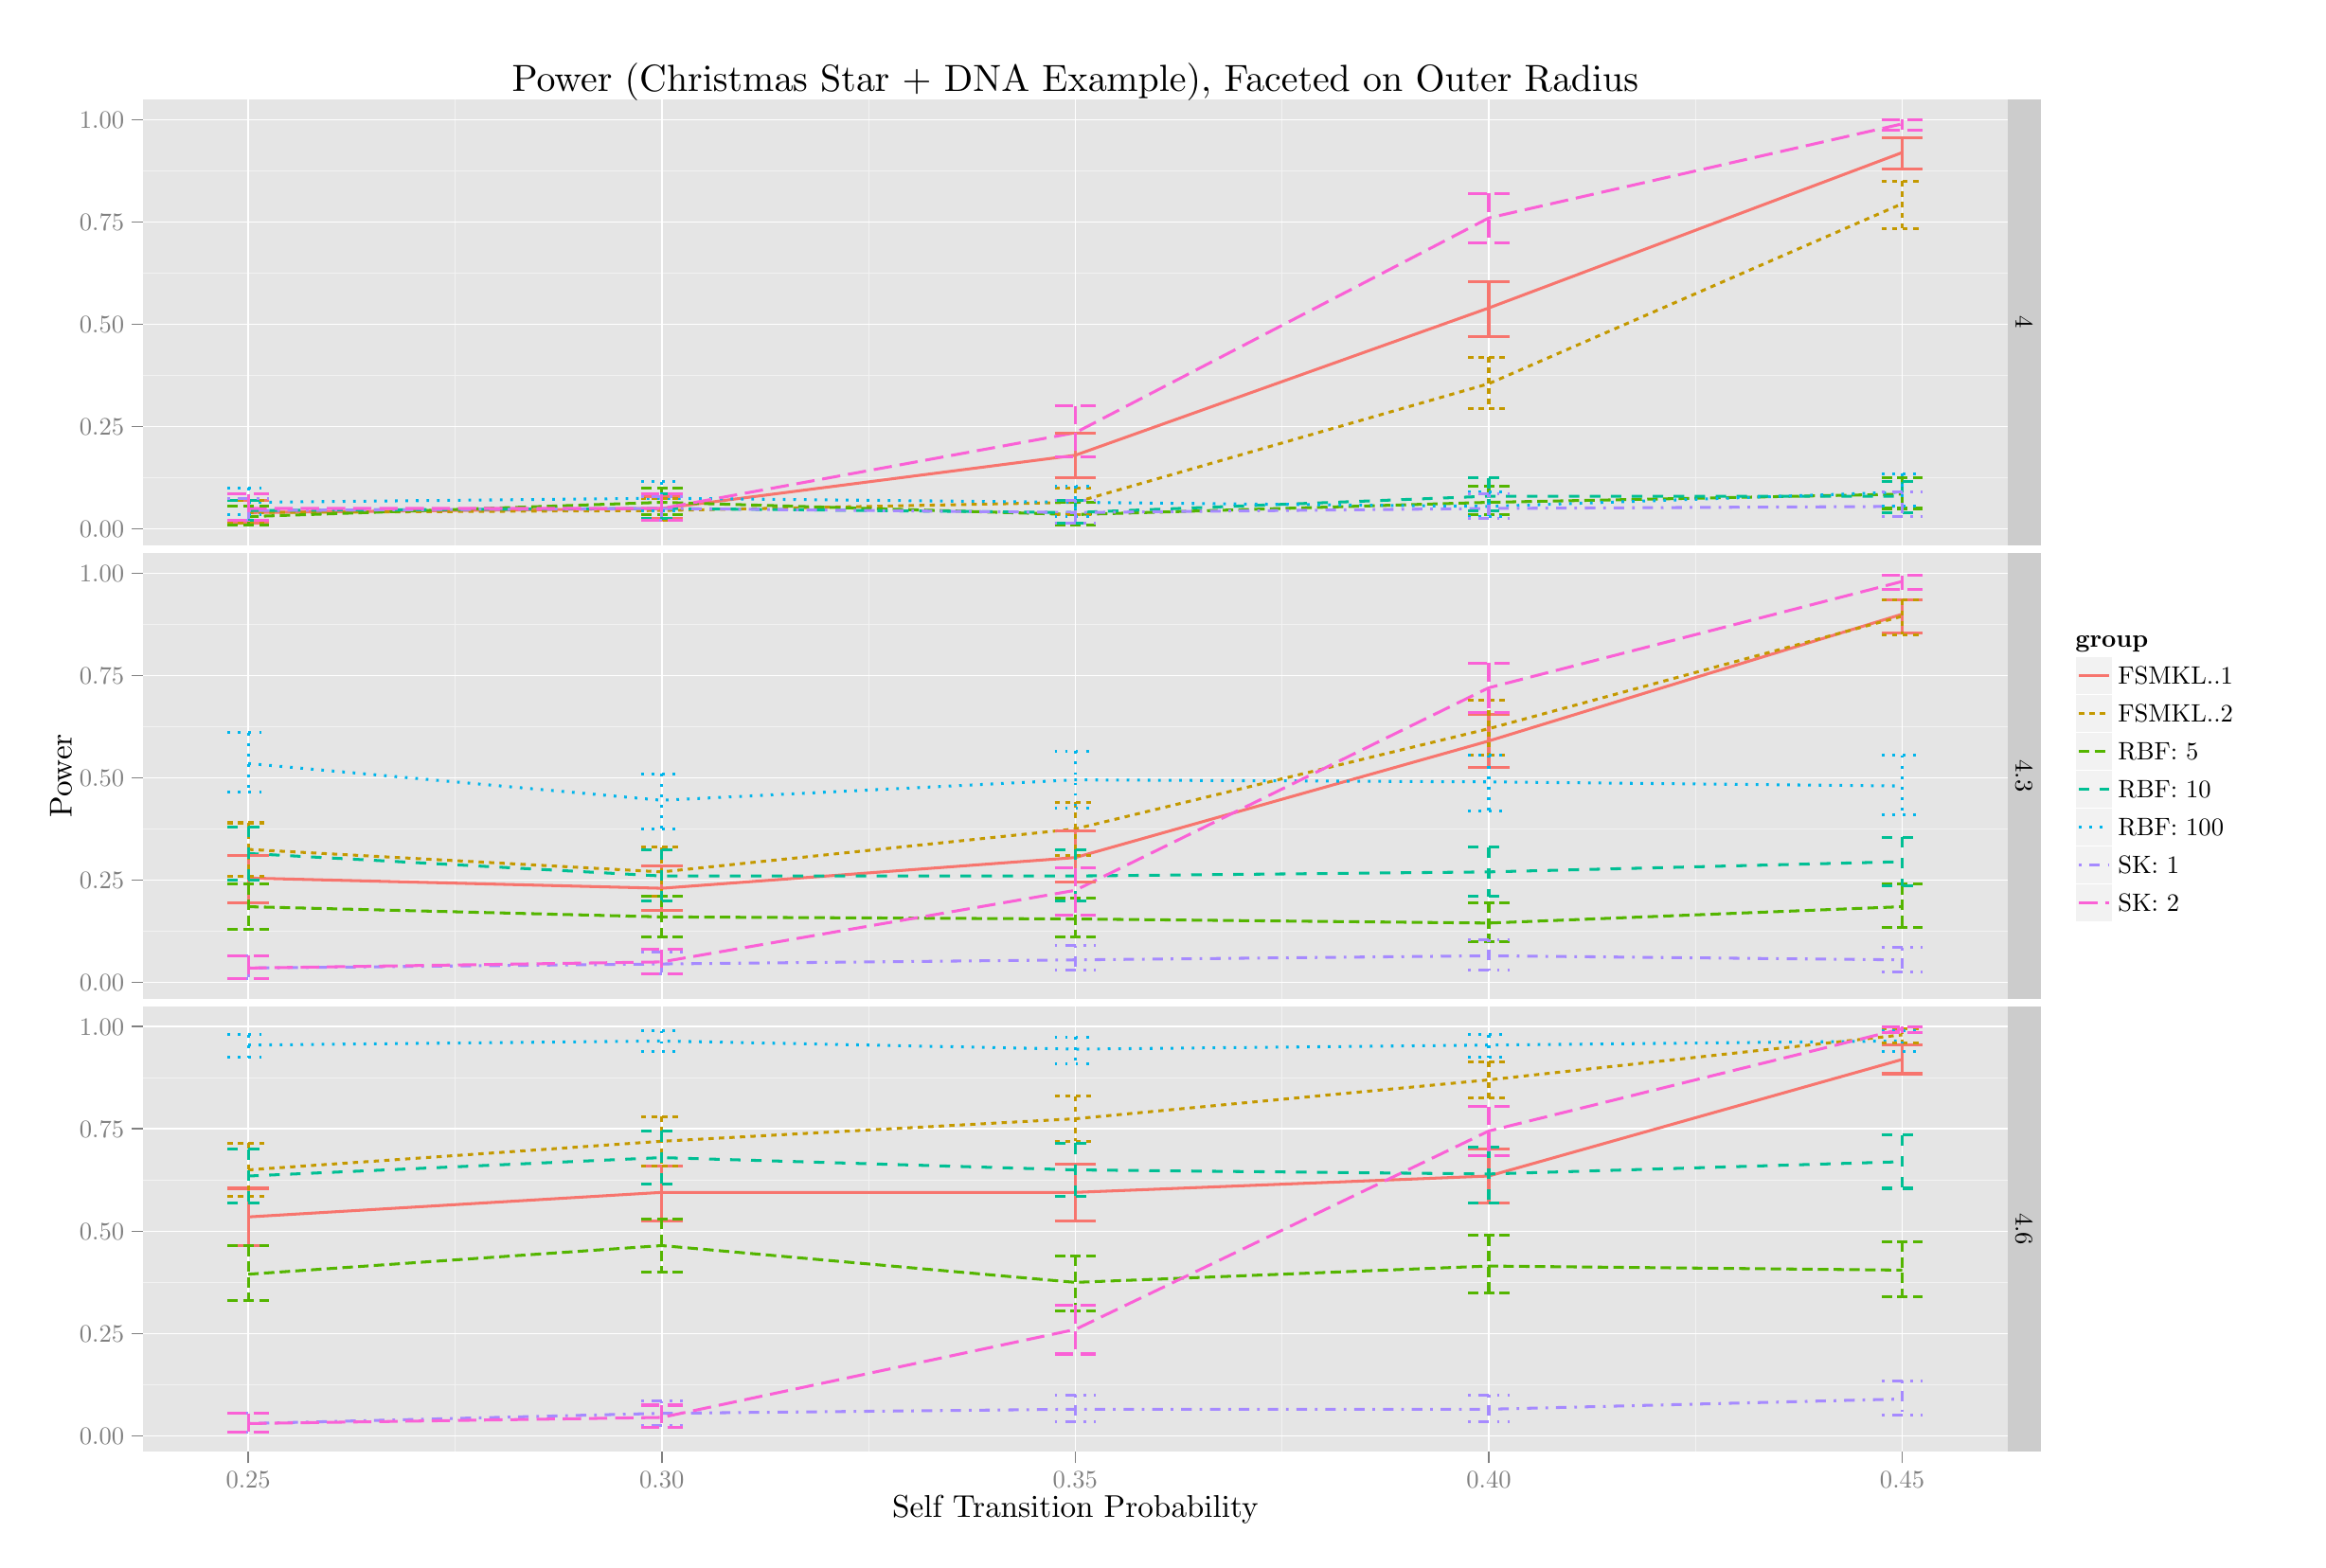
\begin{tikzpicture}[x=1pt,y=1pt]
\definecolor[named]{fillColor}{rgb}{1.00,1.00,1.00}
\path[use as bounding box,fill=fillColor,fill opacity=0.00] (0,0) rectangle (867.24,578.16);
\begin{scope}
\path[clip] (  0.00,  0.00) rectangle (867.24,578.16);
\definecolor[named]{drawColor}{rgb}{1.00,1.00,1.00}
\definecolor[named]{fillColor}{rgb}{1.00,1.00,1.00}

\path[draw=drawColor,line width= 0.6pt,line join=round,line cap=round,fill=fillColor] ( -0.00, -0.00) rectangle (867.24,578.16);
\end{scope}
\begin{scope}
\path[clip] ( 44.49,380.14) rectangle (756.04,550.17);
\definecolor[named]{fillColor}{rgb}{0.90,0.90,0.90}

\path[fill=fillColor] ( 44.49,380.14) rectangle (756.04,550.17);
\definecolor[named]{drawColor}{rgb}{0.95,0.95,0.95}

\path[draw=drawColor,line width= 0.3pt,line join=round] ( 44.49,405.82) --
	(756.04,405.82);

\path[draw=drawColor,line width= 0.3pt,line join=round] ( 44.49,444.86) --
	(756.04,444.86);

\path[draw=drawColor,line width= 0.3pt,line join=round] ( 44.49,483.89) --
	(756.04,483.89);

\path[draw=drawColor,line width= 0.3pt,line join=round] ( 44.49,522.93) --
	(756.04,522.93);

\path[draw=drawColor,line width= 0.3pt,line join=round] (163.60,380.14) --
	(163.60,550.17);

\path[draw=drawColor,line width= 0.3pt,line join=round] (321.38,380.14) --
	(321.38,550.17);

\path[draw=drawColor,line width= 0.3pt,line join=round] (479.15,380.14) --
	(479.15,550.17);

\path[draw=drawColor,line width= 0.3pt,line join=round] (636.92,380.14) --
	(636.92,550.17);
\definecolor[named]{drawColor}{rgb}{1.00,1.00,1.00}

\path[draw=drawColor,line width= 0.6pt,line join=round] ( 44.49,386.30) --
	(756.04,386.30);

\path[draw=drawColor,line width= 0.6pt,line join=round] ( 44.49,425.34) --
	(756.04,425.34);

\path[draw=drawColor,line width= 0.6pt,line join=round] ( 44.49,464.37) --
	(756.04,464.37);

\path[draw=drawColor,line width= 0.6pt,line join=round] ( 44.49,503.41) --
	(756.04,503.41);

\path[draw=drawColor,line width= 0.6pt,line join=round] ( 44.49,542.45) --
	(756.04,542.45);

\path[draw=drawColor,line width= 0.6pt,line join=round] ( 84.72,380.14) --
	( 84.72,550.17);

\path[draw=drawColor,line width= 0.6pt,line join=round] (242.49,380.14) --
	(242.49,550.17);

\path[draw=drawColor,line width= 0.6pt,line join=round] (400.26,380.14) --
	(400.26,550.17);

\path[draw=drawColor,line width= 0.6pt,line join=round] (558.03,380.14) --
	(558.03,550.17);

\path[draw=drawColor,line width= 0.6pt,line join=round] (715.81,380.14) --
	(715.81,550.17);
\definecolor[named]{drawColor}{rgb}{0.97,0.46,0.43}

\path[draw=drawColor,line width= 1.1pt,line join=round] ( 84.72,392.55) --
	(242.49,394.11) --
	(400.26,414.41) --
	(558.03,470.62) --
	(715.81,529.95);
\definecolor[named]{drawColor}{rgb}{0.77,0.60,0.00}

\path[draw=drawColor,line width= 1.1pt,dash pattern=on 2pt off 2pt ,line join=round] ( 84.72,392.55) --
	(242.49,393.33) --
	(400.26,396.45) --
	(558.03,441.73) --
	(715.81,510.44);
\definecolor[named]{drawColor}{rgb}{0.33,0.71,0.00}

\path[draw=drawColor,line width= 1.1pt,dash pattern=on 4pt off 2pt ,line join=round] ( 84.72,390.99) --
	(242.49,396.45) --
	(400.26,391.77) --
	(558.03,396.45) --
	(715.81,399.58);
\definecolor[named]{drawColor}{rgb}{0.00,0.75,0.58}

\path[draw=drawColor,line width= 1.1pt,dash pattern=on 4pt off 4pt ,line join=round] ( 84.72,393.33) --
	(242.49,394.11) --
	(400.26,392.55) --
	(558.03,398.79) --
	(715.81,398.79);
\definecolor[named]{drawColor}{rgb}{0.00,0.71,0.92}

\path[draw=drawColor,line width= 1.1pt,dash pattern=on 1pt off 3pt ,line join=round] ( 84.72,396.45) --
	(242.49,398.01) --
	(400.26,396.45) --
	(558.03,394.89) --
	(715.81,400.36);
\definecolor[named]{drawColor}{rgb}{0.65,0.54,1.00}

\path[draw=drawColor,line width= 1.1pt,dash pattern=on 1pt off 3pt on 4pt off 3pt ,line join=round] ( 84.72,393.33) --
	(242.49,394.11) --
	(400.26,392.55) --
	(558.03,394.11) --
	(715.81,394.89);
\definecolor[named]{drawColor}{rgb}{0.98,0.38,0.84}

\path[draw=drawColor,line width= 1.1pt,dash pattern=on 7pt off 3pt ,line join=round] ( 84.72,394.11) --
	(242.49,394.11) --
	(400.26,423.00) --
	(558.03,504.97) --
	(715.81,540.88);
\definecolor[named]{drawColor}{rgb}{0.97,0.46,0.43}

\path[draw=drawColor,line width= 1.1pt,line join=round] ( 76.83,397.23) --
	( 92.61,397.23);

\path[draw=drawColor,line width= 1.1pt,line join=round] ( 84.72,397.23) --
	( 84.72,388.65);

\path[draw=drawColor,line width= 1.1pt,line join=round] ( 76.83,388.65) --
	( 92.61,388.65);

\path[draw=drawColor,line width= 1.1pt,line join=round] (234.60,398.79) --
	(250.38,398.79);

\path[draw=drawColor,line width= 1.1pt,line join=round] (242.49,398.79) --
	(242.49,390.21);

\path[draw=drawColor,line width= 1.1pt,line join=round] (234.60,390.21) --
	(250.38,390.21);

\path[draw=drawColor,line width= 1.1pt,line join=round] (392.37,423.00) --
	(408.15,423.00);

\path[draw=drawColor,line width= 1.1pt,line join=round] (400.26,423.00) --
	(400.26,405.82);

\path[draw=drawColor,line width= 1.1pt,line join=round] (392.37,405.82) --
	(408.15,405.82);

\path[draw=drawColor,line width= 1.1pt,line join=round] (550.15,480.77) --
	(565.92,480.77);

\path[draw=drawColor,line width= 1.1pt,line join=round] (558.03,480.77) --
	(558.03,459.69);

\path[draw=drawColor,line width= 1.1pt,line join=round] (550.15,459.69) --
	(565.92,459.69);

\path[draw=drawColor,line width= 1.1pt,line join=round] (707.92,535.42) --
	(723.70,535.42);

\path[draw=drawColor,line width= 1.1pt,line join=round] (715.81,535.42) --
	(715.81,523.71);

\path[draw=drawColor,line width= 1.1pt,line join=round] (707.92,523.71) --
	(723.70,523.71);
\definecolor[named]{drawColor}{rgb}{0.77,0.60,0.00}

\path[draw=drawColor,line width= 1.1pt,dash pattern=on 2pt off 2pt ,line join=round] ( 76.83,397.23) --
	( 92.61,397.23);

\path[draw=drawColor,line width= 1.1pt,dash pattern=on 2pt off 2pt ,line join=round] ( 84.72,397.23) --
	( 84.72,388.65);

\path[draw=drawColor,line width= 1.1pt,dash pattern=on 2pt off 2pt ,line join=round] ( 76.83,388.65) --
	( 92.61,388.65);

\path[draw=drawColor,line width= 1.1pt,dash pattern=on 2pt off 2pt ,line join=round] (234.60,398.01) --
	(250.38,398.01);

\path[draw=drawColor,line width= 1.1pt,dash pattern=on 2pt off 2pt ,line join=round] (242.49,398.01) --
	(242.49,389.43);

\path[draw=drawColor,line width= 1.1pt,dash pattern=on 2pt off 2pt ,line join=round] (234.60,389.43) --
	(250.38,389.43);

\path[draw=drawColor,line width= 1.1pt,dash pattern=on 2pt off 2pt ,line join=round] (392.37,401.92) --
	(408.15,401.92);

\path[draw=drawColor,line width= 1.1pt,dash pattern=on 2pt off 2pt ,line join=round] (400.26,401.92) --
	(400.26,391.77);

\path[draw=drawColor,line width= 1.1pt,dash pattern=on 2pt off 2pt ,line join=round] (392.37,391.77) --
	(408.15,391.77);

\path[draw=drawColor,line width= 1.1pt,dash pattern=on 2pt off 2pt ,line join=round] (550.15,451.90) --
	(565.92,451.90);

\path[draw=drawColor,line width= 1.1pt,dash pattern=on 2pt off 2pt ,line join=round] (558.03,451.90) --
	(558.03,432.35);

\path[draw=drawColor,line width= 1.1pt,dash pattern=on 2pt off 2pt ,line join=round] (550.15,432.35) --
	(565.92,432.35);

\path[draw=drawColor,line width= 1.1pt,dash pattern=on 2pt off 2pt ,line join=round] (707.92,519.02) --
	(723.70,519.02);

\path[draw=drawColor,line width= 1.1pt,dash pattern=on 2pt off 2pt ,line join=round] (715.81,519.02) --
	(715.81,501.05);

\path[draw=drawColor,line width= 1.1pt,dash pattern=on 2pt off 2pt ,line join=round] (707.92,501.05) --
	(723.70,501.05);
\definecolor[named]{drawColor}{rgb}{0.33,0.71,0.00}

\path[draw=drawColor,line width= 1.1pt,dash pattern=on 4pt off 2pt ,line join=round] ( 76.83,394.89) --
	( 92.61,394.89);

\path[draw=drawColor,line width= 1.1pt,dash pattern=on 4pt off 2pt ,line join=round] ( 84.72,394.89) --
	( 84.72,387.86);

\path[draw=drawColor,line width= 1.1pt,dash pattern=on 4pt off 2pt ,line join=round] ( 76.83,387.86) --
	( 92.61,387.86);

\path[draw=drawColor,line width= 1.1pt,dash pattern=on 4pt off 2pt ,line join=round] (234.60,401.94) --
	(250.38,401.94);

\path[draw=drawColor,line width= 1.1pt,dash pattern=on 4pt off 2pt ,line join=round] (242.49,401.94) --
	(242.49,391.75);

\path[draw=drawColor,line width= 1.1pt,dash pattern=on 4pt off 2pt ,line join=round] (234.60,391.75) --
	(250.38,391.75);

\path[draw=drawColor,line width= 1.1pt,dash pattern=on 4pt off 2pt ,line join=round] (392.37,396.45) --
	(408.15,396.45);

\path[draw=drawColor,line width= 1.1pt,dash pattern=on 4pt off 2pt ,line join=round] (400.26,396.45) --
	(400.26,387.86);

\path[draw=drawColor,line width= 1.1pt,dash pattern=on 4pt off 2pt ,line join=round] (392.37,387.86) --
	(408.15,387.86);

\path[draw=drawColor,line width= 1.1pt,dash pattern=on 4pt off 2pt ,line join=round] (550.15,402.70) --
	(565.92,402.70);

\path[draw=drawColor,line width= 1.1pt,dash pattern=on 4pt off 2pt ,line join=round] (558.03,402.70) --
	(558.03,391.77);

\path[draw=drawColor,line width= 1.1pt,dash pattern=on 4pt off 2pt ,line join=round] (550.15,391.77) --
	(565.92,391.77);

\path[draw=drawColor,line width= 1.1pt,dash pattern=on 4pt off 2pt ,line join=round] (707.92,405.82) --
	(723.70,405.82);

\path[draw=drawColor,line width= 1.1pt,dash pattern=on 4pt off 2pt ,line join=round] (715.81,405.82) --
	(715.81,394.11);

\path[draw=drawColor,line width= 1.1pt,dash pattern=on 4pt off 2pt ,line join=round] (707.92,394.11) --
	(723.70,394.11);
\definecolor[named]{drawColor}{rgb}{0.00,0.75,0.58}

\path[draw=drawColor,line width= 1.1pt,dash pattern=on 4pt off 4pt ,line join=round] ( 76.83,397.25) --
	( 92.61,397.25);

\path[draw=drawColor,line width= 1.1pt,dash pattern=on 4pt off 4pt ,line join=round] ( 84.72,397.25) --
	( 84.72,389.43);

\path[draw=drawColor,line width= 1.1pt,dash pattern=on 4pt off 4pt ,line join=round] ( 76.83,389.43) --
	( 92.61,389.43);

\path[draw=drawColor,line width= 1.1pt,dash pattern=on 4pt off 4pt ,line join=round] (234.60,399.58) --
	(250.38,399.58);

\path[draw=drawColor,line width= 1.1pt,dash pattern=on 4pt off 4pt ,line join=round] (242.49,399.58) --
	(242.49,390.21);

\path[draw=drawColor,line width= 1.1pt,dash pattern=on 4pt off 4pt ,line join=round] (234.60,390.21) --
	(250.38,390.21);

\path[draw=drawColor,line width= 1.1pt,dash pattern=on 4pt off 4pt ,line join=round] (392.37,397.23) --
	(408.15,397.23);

\path[draw=drawColor,line width= 1.1pt,dash pattern=on 4pt off 4pt ,line join=round] (400.26,397.23) --
	(400.26,388.65);

\path[draw=drawColor,line width= 1.1pt,dash pattern=on 4pt off 4pt ,line join=round] (392.37,388.65) --
	(408.15,388.65);

\path[draw=drawColor,line width= 1.1pt,dash pattern=on 4pt off 4pt ,line join=round] (550.15,405.82) --
	(565.92,405.82);

\path[draw=drawColor,line width= 1.1pt,dash pattern=on 4pt off 4pt ,line join=round] (558.03,405.82) --
	(558.03,393.33);

\path[draw=drawColor,line width= 1.1pt,dash pattern=on 4pt off 4pt ,line join=round] (550.15,393.33) --
	(565.92,393.33);

\path[draw=drawColor,line width= 1.1pt,dash pattern=on 4pt off 4pt ,line join=round] (707.92,404.26) --
	(723.70,404.26);

\path[draw=drawColor,line width= 1.1pt,dash pattern=on 4pt off 4pt ,line join=round] (715.81,404.26) --
	(715.81,392.55);

\path[draw=drawColor,line width= 1.1pt,dash pattern=on 4pt off 4pt ,line join=round] (707.92,392.55) --
	(723.70,392.55);
\definecolor[named]{drawColor}{rgb}{0.00,0.71,0.92}

\path[draw=drawColor,line width= 1.1pt,dash pattern=on 1pt off 3pt ,line join=round] ( 76.83,401.92) --
	( 92.61,401.92);

\path[draw=drawColor,line width= 1.1pt,dash pattern=on 1pt off 3pt ,line join=round] ( 84.72,401.92) --
	( 84.72,391.75);

\path[draw=drawColor,line width= 1.1pt,dash pattern=on 1pt off 3pt ,line join=round] ( 76.83,391.75) --
	( 92.61,391.75);

\path[draw=drawColor,line width= 1.1pt,dash pattern=on 1pt off 3pt ,line join=round] (234.60,404.26) --
	(250.38,404.26);

\path[draw=drawColor,line width= 1.1pt,dash pattern=on 1pt off 3pt ,line join=round] (242.49,404.26) --
	(242.49,393.33);

\path[draw=drawColor,line width= 1.1pt,dash pattern=on 1pt off 3pt ,line join=round] (234.60,393.33) --
	(250.38,393.33);

\path[draw=drawColor,line width= 1.1pt,dash pattern=on 1pt off 3pt ,line join=round] (392.37,402.70) --
	(408.15,402.70);

\path[draw=drawColor,line width= 1.1pt,dash pattern=on 1pt off 3pt ,line join=round] (400.26,402.70) --
	(400.26,390.99);

\path[draw=drawColor,line width= 1.1pt,dash pattern=on 1pt off 3pt ,line join=round] (392.37,390.99) --
	(408.15,390.99);

\path[draw=drawColor,line width= 1.1pt,dash pattern=on 1pt off 3pt ,line join=round] (550.15,400.36) --
	(565.92,400.36);

\path[draw=drawColor,line width= 1.1pt,dash pattern=on 1pt off 3pt ,line join=round] (558.03,400.36) --
	(558.03,390.97);

\path[draw=drawColor,line width= 1.1pt,dash pattern=on 1pt off 3pt ,line join=round] (550.15,390.97) --
	(565.92,390.97);

\path[draw=drawColor,line width= 1.1pt,dash pattern=on 1pt off 3pt ,line join=round] (707.92,407.38) --
	(723.70,407.38);

\path[draw=drawColor,line width= 1.1pt,dash pattern=on 1pt off 3pt ,line join=round] (715.81,407.38) --
	(715.81,394.87);

\path[draw=drawColor,line width= 1.1pt,dash pattern=on 1pt off 3pt ,line join=round] (707.92,394.87) --
	(723.70,394.87);
\definecolor[named]{drawColor}{rgb}{0.65,0.54,1.00}

\path[draw=drawColor,line width= 1.1pt,dash pattern=on 1pt off 3pt on 4pt off 3pt ,line join=round] ( 76.83,398.01) --
	( 92.61,398.01);

\path[draw=drawColor,line width= 1.1pt,dash pattern=on 1pt off 3pt on 4pt off 3pt ,line join=round] ( 84.72,398.01) --
	( 84.72,389.43);

\path[draw=drawColor,line width= 1.1pt,dash pattern=on 1pt off 3pt on 4pt off 3pt ,line join=round] ( 76.83,389.43) --
	( 92.61,389.43);

\path[draw=drawColor,line width= 1.1pt,dash pattern=on 1pt off 3pt on 4pt off 3pt ,line join=round] (234.60,398.79) --
	(250.38,398.79);

\path[draw=drawColor,line width= 1.1pt,dash pattern=on 1pt off 3pt on 4pt off 3pt ,line join=round] (242.49,398.79) --
	(242.49,389.43);

\path[draw=drawColor,line width= 1.1pt,dash pattern=on 1pt off 3pt on 4pt off 3pt ,line join=round] (234.60,389.43) --
	(250.38,389.43);

\path[draw=drawColor,line width= 1.1pt,dash pattern=on 1pt off 3pt on 4pt off 3pt ,line join=round] (392.37,397.23) --
	(408.15,397.23);

\path[draw=drawColor,line width= 1.1pt,dash pattern=on 1pt off 3pt on 4pt off 3pt ,line join=round] (400.26,397.23) --
	(400.26,388.65);

\path[draw=drawColor,line width= 1.1pt,dash pattern=on 1pt off 3pt on 4pt off 3pt ,line join=round] (392.37,388.65) --
	(408.15,388.65);

\path[draw=drawColor,line width= 1.1pt,dash pattern=on 1pt off 3pt on 4pt off 3pt ,line join=round] (550.15,399.58) --
	(565.92,399.58);

\path[draw=drawColor,line width= 1.1pt,dash pattern=on 1pt off 3pt on 4pt off 3pt ,line join=round] (558.03,399.58) --
	(558.03,390.19);

\path[draw=drawColor,line width= 1.1pt,dash pattern=on 1pt off 3pt on 4pt off 3pt ,line join=round] (550.15,390.19) --
	(565.92,390.19);

\path[draw=drawColor,line width= 1.1pt,dash pattern=on 1pt off 3pt on 4pt off 3pt ,line join=round] (707.92,400.36) --
	(723.70,400.36);

\path[draw=drawColor,line width= 1.1pt,dash pattern=on 1pt off 3pt on 4pt off 3pt ,line join=round] (715.81,400.36) --
	(715.81,390.99);

\path[draw=drawColor,line width= 1.1pt,dash pattern=on 1pt off 3pt on 4pt off 3pt ,line join=round] (707.92,390.99) --
	(723.70,390.99);
\definecolor[named]{drawColor}{rgb}{0.98,0.38,0.84}

\path[draw=drawColor,line width= 1.1pt,dash pattern=on 7pt off 3pt ,line join=round] ( 76.83,399.58) --
	( 92.61,399.58);

\path[draw=drawColor,line width= 1.1pt,dash pattern=on 7pt off 3pt ,line join=round] ( 84.72,399.58) --
	( 84.72,389.43);

\path[draw=drawColor,line width= 1.1pt,dash pattern=on 7pt off 3pt ,line join=round] ( 76.83,389.43) --
	( 92.61,389.43);

\path[draw=drawColor,line width= 1.1pt,dash pattern=on 7pt off 3pt ,line join=round] (234.60,399.58) --
	(250.38,399.58);

\path[draw=drawColor,line width= 1.1pt,dash pattern=on 7pt off 3pt ,line join=round] (242.49,399.58) --
	(242.49,389.43);

\path[draw=drawColor,line width= 1.1pt,dash pattern=on 7pt off 3pt ,line join=round] (234.60,389.43) --
	(250.38,389.43);

\path[draw=drawColor,line width= 1.1pt,dash pattern=on 7pt off 3pt ,line join=round] (392.37,433.15) --
	(408.15,433.15);

\path[draw=drawColor,line width= 1.1pt,dash pattern=on 7pt off 3pt ,line join=round] (400.26,433.15) --
	(400.26,413.63);

\path[draw=drawColor,line width= 1.1pt,dash pattern=on 7pt off 3pt ,line join=round] (392.37,413.63) --
	(408.15,413.63);

\path[draw=drawColor,line width= 1.1pt,dash pattern=on 7pt off 3pt ,line join=round] (550.15,514.34) --
	(565.92,514.34);

\path[draw=drawColor,line width= 1.1pt,dash pattern=on 7pt off 3pt ,line join=round] (558.03,514.34) --
	(558.03,495.60);

\path[draw=drawColor,line width= 1.1pt,dash pattern=on 7pt off 3pt ,line join=round] (550.15,495.60) --
	(565.92,495.60);

\path[draw=drawColor,line width= 1.1pt,dash pattern=on 7pt off 3pt ,line join=round] (707.92,542.45) --
	(723.70,542.45);

\path[draw=drawColor,line width= 1.1pt,dash pattern=on 7pt off 3pt ,line join=round] (715.81,542.45) --
	(715.81,538.54);

\path[draw=drawColor,line width= 1.1pt,dash pattern=on 7pt off 3pt ,line join=round] (707.92,538.54) --
	(723.70,538.54);
\end{scope}
\begin{scope}
\path[clip] ( 44.49,207.09) rectangle (756.04,377.12);
\definecolor[named]{fillColor}{rgb}{0.90,0.90,0.90}

\path[fill=fillColor] ( 44.49,207.09) rectangle (756.04,377.12);
\definecolor[named]{drawColor}{rgb}{0.95,0.95,0.95}

\path[draw=drawColor,line width= 0.3pt,line join=round] ( 44.49,232.77) --
	(756.04,232.77);

\path[draw=drawColor,line width= 0.3pt,line join=round] ( 44.49,271.81) --
	(756.04,271.81);

\path[draw=drawColor,line width= 0.3pt,line join=round] ( 44.49,310.84) --
	(756.04,310.84);

\path[draw=drawColor,line width= 0.3pt,line join=round] ( 44.49,349.88) --
	(756.04,349.88);

\path[draw=drawColor,line width= 0.3pt,line join=round] (163.60,207.09) --
	(163.60,377.12);

\path[draw=drawColor,line width= 0.3pt,line join=round] (321.38,207.09) --
	(321.38,377.12);

\path[draw=drawColor,line width= 0.3pt,line join=round] (479.15,207.09) --
	(479.15,377.12);

\path[draw=drawColor,line width= 0.3pt,line join=round] (636.92,207.09) --
	(636.92,377.12);
\definecolor[named]{drawColor}{rgb}{1.00,1.00,1.00}

\path[draw=drawColor,line width= 0.6pt,line join=round] ( 44.49,213.25) --
	(756.04,213.25);

\path[draw=drawColor,line width= 0.6pt,line join=round] ( 44.49,252.29) --
	(756.04,252.29);

\path[draw=drawColor,line width= 0.6pt,line join=round] ( 44.49,291.32) --
	(756.04,291.32);

\path[draw=drawColor,line width= 0.6pt,line join=round] ( 44.49,330.36) --
	(756.04,330.36);

\path[draw=drawColor,line width= 0.6pt,line join=round] ( 44.49,369.40) --
	(756.04,369.40);

\path[draw=drawColor,line width= 0.6pt,line join=round] ( 84.72,207.09) --
	( 84.72,377.12);

\path[draw=drawColor,line width= 0.6pt,line join=round] (242.49,207.09) --
	(242.49,377.12);

\path[draw=drawColor,line width= 0.6pt,line join=round] (400.26,207.09) --
	(400.26,377.12);

\path[draw=drawColor,line width= 0.6pt,line join=round] (558.03,207.09) --
	(558.03,377.12);

\path[draw=drawColor,line width= 0.6pt,line join=round] (715.81,207.09) --
	(715.81,377.12);
\definecolor[named]{drawColor}{rgb}{0.97,0.46,0.43}

\path[draw=drawColor,line width= 1.1pt,line join=round] ( 84.72,253.07) --
	(242.49,249.17) --
	(400.26,260.88) --
	(558.03,305.38) --
	(715.81,353.78);
\definecolor[named]{drawColor}{rgb}{0.77,0.60,0.00}

\path[draw=drawColor,line width= 1.1pt,dash pattern=on 2pt off 2pt ,line join=round] ( 84.72,264.00) --
	(242.49,255.41) --
	(400.26,271.81) --
	(558.03,310.06) --
	(715.81,353.00);
\definecolor[named]{drawColor}{rgb}{0.33,0.71,0.00}

\path[draw=drawColor,line width= 1.1pt,dash pattern=on 4pt off 2pt ,line join=round] ( 84.72,242.14) --
	(242.49,238.24) --
	(400.26,237.45) --
	(558.03,235.89) --
	(715.81,242.14);
\definecolor[named]{drawColor}{rgb}{0.00,0.75,0.58}

\path[draw=drawColor,line width= 1.1pt,dash pattern=on 4pt off 4pt ,line join=round] ( 84.72,262.44) --
	(242.49,253.85) --
	(400.26,253.85) --
	(558.03,255.41) --
	(715.81,259.31);
\definecolor[named]{drawColor}{rgb}{0.00,0.71,0.92}

\path[draw=drawColor,line width= 1.1pt,dash pattern=on 1pt off 3pt ,line join=round] ( 84.72,296.79) --
	(242.49,282.74) --
	(400.26,290.54) --
	(558.03,289.76) --
	(715.81,288.20);
\definecolor[named]{drawColor}{rgb}{0.65,0.54,1.00}

\path[draw=drawColor,line width= 1.1pt,dash pattern=on 1pt off 3pt on 4pt off 3pt ,line join=round] ( 84.72,218.72) --
	(242.49,220.28) --
	(400.26,221.84) --
	(558.03,223.40) --
	(715.81,221.84);
\definecolor[named]{drawColor}{rgb}{0.98,0.38,0.84}

\path[draw=drawColor,line width= 1.1pt,dash pattern=on 7pt off 3pt ,line join=round] ( 84.72,218.72) --
	(242.49,221.06) --
	(400.26,248.38) --
	(558.03,325.68) --
	(715.81,366.27);
\definecolor[named]{drawColor}{rgb}{0.97,0.46,0.43}

\path[draw=drawColor,line width= 1.1pt,line join=round] ( 76.83,261.66) --
	( 92.61,261.66);

\path[draw=drawColor,line width= 1.1pt,line join=round] ( 84.72,261.66) --
	( 84.72,243.70);

\path[draw=drawColor,line width= 1.1pt,line join=round] ( 76.83,243.70) --
	( 92.61,243.70);

\path[draw=drawColor,line width= 1.1pt,line join=round] (234.60,257.75) --
	(250.38,257.75);

\path[draw=drawColor,line width= 1.1pt,line join=round] (242.49,257.75) --
	(242.49,240.58);

\path[draw=drawColor,line width= 1.1pt,line join=round] (234.60,240.58) --
	(250.38,240.58);

\path[draw=drawColor,line width= 1.1pt,line join=round] (392.37,271.03) --
	(408.15,271.03);

\path[draw=drawColor,line width= 1.1pt,line join=round] (400.26,271.03) --
	(400.26,251.51);

\path[draw=drawColor,line width= 1.1pt,line join=round] (392.37,251.51) --
	(408.15,251.51);

\path[draw=drawColor,line width= 1.1pt,line join=round] (550.15,315.53) --
	(565.92,315.53);

\path[draw=drawColor,line width= 1.1pt,line join=round] (558.03,315.53) --
	(558.03,295.23);

\path[draw=drawColor,line width= 1.1pt,line join=round] (550.15,295.23) --
	(565.92,295.23);

\path[draw=drawColor,line width= 1.1pt,line join=round] (707.92,359.25) --
	(723.70,359.25);

\path[draw=drawColor,line width= 1.1pt,line join=round] (715.81,359.25) --
	(715.81,346.75);

\path[draw=drawColor,line width= 1.1pt,line join=round] (707.92,346.75) --
	(723.70,346.75);
\definecolor[named]{drawColor}{rgb}{0.77,0.60,0.00}

\path[draw=drawColor,line width= 1.1pt,dash pattern=on 2pt off 2pt ,line join=round] ( 76.83,274.15) --
	( 92.61,274.15);

\path[draw=drawColor,line width= 1.1pt,dash pattern=on 2pt off 2pt ,line join=round] ( 84.72,274.15) --
	( 84.72,253.85);

\path[draw=drawColor,line width= 1.1pt,dash pattern=on 2pt off 2pt ,line join=round] ( 76.83,253.85) --
	( 92.61,253.85);

\path[draw=drawColor,line width= 1.1pt,dash pattern=on 2pt off 2pt ,line join=round] (234.60,264.78) --
	(250.38,264.78);

\path[draw=drawColor,line width= 1.1pt,dash pattern=on 2pt off 2pt ,line join=round] (242.49,264.78) --
	(242.49,246.04);

\path[draw=drawColor,line width= 1.1pt,dash pattern=on 2pt off 2pt ,line join=round] (234.60,246.04) --
	(250.38,246.04);

\path[draw=drawColor,line width= 1.1pt,dash pattern=on 2pt off 2pt ,line join=round] (392.37,281.96) --
	(408.15,281.96);

\path[draw=drawColor,line width= 1.1pt,dash pattern=on 2pt off 2pt ,line join=round] (400.26,281.96) --
	(400.26,261.66);

\path[draw=drawColor,line width= 1.1pt,dash pattern=on 2pt off 2pt ,line join=round] (392.37,261.66) --
	(408.15,261.66);

\path[draw=drawColor,line width= 1.1pt,dash pattern=on 2pt off 2pt ,line join=round] (550.15,320.99) --
	(565.92,320.99);

\path[draw=drawColor,line width= 1.1pt,dash pattern=on 2pt off 2pt ,line join=round] (558.03,320.99) --
	(558.03,299.89);

\path[draw=drawColor,line width= 1.1pt,dash pattern=on 2pt off 2pt ,line join=round] (550.15,299.89) --
	(565.92,299.89);

\path[draw=drawColor,line width= 1.1pt,dash pattern=on 2pt off 2pt ,line join=round] (707.92,359.25) --
	(723.70,359.25);

\path[draw=drawColor,line width= 1.1pt,dash pattern=on 2pt off 2pt ,line join=round] (715.81,359.25) --
	(715.81,345.97);

\path[draw=drawColor,line width= 1.1pt,dash pattern=on 2pt off 2pt ,line join=round] (707.92,345.97) --
	(723.70,345.97);
\definecolor[named]{drawColor}{rgb}{0.33,0.71,0.00}

\path[draw=drawColor,line width= 1.1pt,dash pattern=on 4pt off 2pt ,line join=round] ( 76.83,250.73) --
	( 92.61,250.73);

\path[draw=drawColor,line width= 1.1pt,dash pattern=on 4pt off 2pt ,line join=round] ( 84.72,250.73) --
	( 84.72,233.55);

\path[draw=drawColor,line width= 1.1pt,dash pattern=on 4pt off 2pt ,line join=round] ( 76.83,233.55) --
	( 92.61,233.55);

\path[draw=drawColor,line width= 1.1pt,dash pattern=on 4pt off 2pt ,line join=round] (234.60,246.04) --
	(250.38,246.04);

\path[draw=drawColor,line width= 1.1pt,dash pattern=on 4pt off 2pt ,line join=round] (242.49,246.04) --
	(242.49,230.43);

\path[draw=drawColor,line width= 1.1pt,dash pattern=on 4pt off 2pt ,line join=round] (234.60,230.43) --
	(250.38,230.43);

\path[draw=drawColor,line width= 1.1pt,dash pattern=on 4pt off 2pt ,line join=round] (392.37,245.26) --
	(408.15,245.26);

\path[draw=drawColor,line width= 1.1pt,dash pattern=on 4pt off 2pt ,line join=round] (400.26,245.26) --
	(400.26,230.43);

\path[draw=drawColor,line width= 1.1pt,dash pattern=on 4pt off 2pt ,line join=round] (392.37,230.43) --
	(408.15,230.43);

\path[draw=drawColor,line width= 1.1pt,dash pattern=on 4pt off 2pt ,line join=round] (550.15,243.70) --
	(565.92,243.70);

\path[draw=drawColor,line width= 1.1pt,dash pattern=on 4pt off 2pt ,line join=round] (558.03,243.70) --
	(558.03,228.85);

\path[draw=drawColor,line width= 1.1pt,dash pattern=on 4pt off 2pt ,line join=round] (550.15,228.85) --
	(565.92,228.85);

\path[draw=drawColor,line width= 1.1pt,dash pattern=on 4pt off 2pt ,line join=round] (707.92,250.73) --
	(723.70,250.73);

\path[draw=drawColor,line width= 1.1pt,dash pattern=on 4pt off 2pt ,line join=round] (715.81,250.73) --
	(715.81,234.33);

\path[draw=drawColor,line width= 1.1pt,dash pattern=on 4pt off 2pt ,line join=round] (707.92,234.33) --
	(723.70,234.33);
\definecolor[named]{drawColor}{rgb}{0.00,0.75,0.58}

\path[draw=drawColor,line width= 1.1pt,dash pattern=on 4pt off 4pt ,line join=round] ( 76.83,272.59) --
	( 92.61,272.59);

\path[draw=drawColor,line width= 1.1pt,dash pattern=on 4pt off 4pt ,line join=round] ( 84.72,272.59) --
	( 84.72,252.29);

\path[draw=drawColor,line width= 1.1pt,dash pattern=on 4pt off 4pt ,line join=round] ( 76.83,252.29) --
	( 92.61,252.29);

\path[draw=drawColor,line width= 1.1pt,dash pattern=on 4pt off 4pt ,line join=round] (234.60,264.00) --
	(250.38,264.00);

\path[draw=drawColor,line width= 1.1pt,dash pattern=on 4pt off 4pt ,line join=round] (242.49,264.00) --
	(242.49,244.48);

\path[draw=drawColor,line width= 1.1pt,dash pattern=on 4pt off 4pt ,line join=round] (234.60,244.48) --
	(250.38,244.48);

\path[draw=drawColor,line width= 1.1pt,dash pattern=on 4pt off 4pt ,line join=round] (392.37,264.00) --
	(408.15,264.00);

\path[draw=drawColor,line width= 1.1pt,dash pattern=on 4pt off 4pt ,line join=round] (400.26,264.00) --
	(400.26,244.48);

\path[draw=drawColor,line width= 1.1pt,dash pattern=on 4pt off 4pt ,line join=round] (392.37,244.48) --
	(408.15,244.48);

\path[draw=drawColor,line width= 1.1pt,dash pattern=on 4pt off 4pt ,line join=round] (550.15,264.80) --
	(565.92,264.80);

\path[draw=drawColor,line width= 1.1pt,dash pattern=on 4pt off 4pt ,line join=round] (558.03,264.80) --
	(558.03,246.04);

\path[draw=drawColor,line width= 1.1pt,dash pattern=on 4pt off 4pt ,line join=round] (550.15,246.04) --
	(565.92,246.04);

\path[draw=drawColor,line width= 1.1pt,dash pattern=on 4pt off 4pt ,line join=round] (707.92,268.68) --
	(723.70,268.68);

\path[draw=drawColor,line width= 1.1pt,dash pattern=on 4pt off 4pt ,line join=round] (715.81,268.68) --
	(715.81,249.95);

\path[draw=drawColor,line width= 1.1pt,dash pattern=on 4pt off 4pt ,line join=round] (707.92,249.95) --
	(723.70,249.95);
\definecolor[named]{drawColor}{rgb}{0.00,0.71,0.92}

\path[draw=drawColor,line width= 1.1pt,dash pattern=on 1pt off 3pt ,line join=round] ( 76.83,308.50) --
	( 92.61,308.50);

\path[draw=drawColor,line width= 1.1pt,dash pattern=on 1pt off 3pt ,line join=round] ( 84.72,308.50) --
	( 84.72,285.86);

\path[draw=drawColor,line width= 1.1pt,dash pattern=on 1pt off 3pt ,line join=round] ( 76.83,285.86) --
	( 92.61,285.86);

\path[draw=drawColor,line width= 1.1pt,dash pattern=on 1pt off 3pt ,line join=round] (234.60,292.90) --
	(250.38,292.90);

\path[draw=drawColor,line width= 1.1pt,dash pattern=on 1pt off 3pt ,line join=round] (242.49,292.90) --
	(242.49,271.79);

\path[draw=drawColor,line width= 1.1pt,dash pattern=on 1pt off 3pt ,line join=round] (234.60,271.79) --
	(250.38,271.79);

\path[draw=drawColor,line width= 1.1pt,dash pattern=on 1pt off 3pt ,line join=round] (392.37,301.47) --
	(408.15,301.47);

\path[draw=drawColor,line width= 1.1pt,dash pattern=on 1pt off 3pt ,line join=round] (400.26,301.47) --
	(400.26,279.61);

\path[draw=drawColor,line width= 1.1pt,dash pattern=on 1pt off 3pt ,line join=round] (392.37,279.61) --
	(408.15,279.61);

\path[draw=drawColor,line width= 1.1pt,dash pattern=on 1pt off 3pt ,line join=round] (550.15,299.91) --
	(565.92,299.91);

\path[draw=drawColor,line width= 1.1pt,dash pattern=on 1pt off 3pt ,line join=round] (558.03,299.91) --
	(558.03,278.83);

\path[draw=drawColor,line width= 1.1pt,dash pattern=on 1pt off 3pt ,line join=round] (550.15,278.83) --
	(565.92,278.83);

\path[draw=drawColor,line width= 1.1pt,dash pattern=on 1pt off 3pt ,line join=round] (707.92,299.91) --
	(723.70,299.91);

\path[draw=drawColor,line width= 1.1pt,dash pattern=on 1pt off 3pt ,line join=round] (715.81,299.91) --
	(715.81,277.27);

\path[draw=drawColor,line width= 1.1pt,dash pattern=on 1pt off 3pt ,line join=round] (707.92,277.27) --
	(723.70,277.27);
\definecolor[named]{drawColor}{rgb}{0.65,0.54,1.00}

\path[draw=drawColor,line width= 1.1pt,dash pattern=on 1pt off 3pt on 4pt off 3pt ,line join=round] ( 76.83,223.40) --
	( 92.61,223.40);

\path[draw=drawColor,line width= 1.1pt,dash pattern=on 1pt off 3pt on 4pt off 3pt ,line join=round] ( 84.72,223.40) --
	( 84.72,214.81);

\path[draw=drawColor,line width= 1.1pt,dash pattern=on 1pt off 3pt on 4pt off 3pt ,line join=round] ( 76.83,214.81) --
	( 92.61,214.81);

\path[draw=drawColor,line width= 1.1pt,dash pattern=on 1pt off 3pt on 4pt off 3pt ,line join=round] (234.60,224.96) --
	(250.38,224.96);

\path[draw=drawColor,line width= 1.1pt,dash pattern=on 1pt off 3pt on 4pt off 3pt ,line join=round] (242.49,224.96) --
	(242.49,216.38);

\path[draw=drawColor,line width= 1.1pt,dash pattern=on 1pt off 3pt on 4pt off 3pt ,line join=round] (234.60,216.38) --
	(250.38,216.38);

\path[draw=drawColor,line width= 1.1pt,dash pattern=on 1pt off 3pt on 4pt off 3pt ,line join=round] (392.37,227.31) --
	(408.15,227.31);

\path[draw=drawColor,line width= 1.1pt,dash pattern=on 1pt off 3pt on 4pt off 3pt ,line join=round] (400.26,227.31) --
	(400.26,217.94);

\path[draw=drawColor,line width= 1.1pt,dash pattern=on 1pt off 3pt on 4pt off 3pt ,line join=round] (392.37,217.94) --
	(408.15,217.94);

\path[draw=drawColor,line width= 1.1pt,dash pattern=on 1pt off 3pt on 4pt off 3pt ,line join=round] (550.15,229.65) --
	(565.92,229.65);

\path[draw=drawColor,line width= 1.1pt,dash pattern=on 1pt off 3pt on 4pt off 3pt ,line join=round] (558.03,229.65) --
	(558.03,217.94);

\path[draw=drawColor,line width= 1.1pt,dash pattern=on 1pt off 3pt on 4pt off 3pt ,line join=round] (550.15,217.94) --
	(565.92,217.94);

\path[draw=drawColor,line width= 1.1pt,dash pattern=on 1pt off 3pt on 4pt off 3pt ,line join=round] (707.92,226.52) --
	(723.70,226.52);

\path[draw=drawColor,line width= 1.1pt,dash pattern=on 1pt off 3pt on 4pt off 3pt ,line join=round] (715.81,226.52) --
	(715.81,217.16);

\path[draw=drawColor,line width= 1.1pt,dash pattern=on 1pt off 3pt on 4pt off 3pt ,line join=round] (707.92,217.16) --
	(723.70,217.16);
\definecolor[named]{drawColor}{rgb}{0.98,0.38,0.84}

\path[draw=drawColor,line width= 1.1pt,dash pattern=on 7pt off 3pt ,line join=round] ( 76.83,223.40) --
	( 92.61,223.40);

\path[draw=drawColor,line width= 1.1pt,dash pattern=on 7pt off 3pt ,line join=round] ( 84.72,223.40) --
	( 84.72,214.81);

\path[draw=drawColor,line width= 1.1pt,dash pattern=on 7pt off 3pt ,line join=round] ( 76.83,214.81) --
	( 92.61,214.81);

\path[draw=drawColor,line width= 1.1pt,dash pattern=on 7pt off 3pt ,line join=round] (234.60,225.74) --
	(250.38,225.74);

\path[draw=drawColor,line width= 1.1pt,dash pattern=on 7pt off 3pt ,line join=round] (242.49,225.74) --
	(242.49,216.38);

\path[draw=drawColor,line width= 1.1pt,dash pattern=on 7pt off 3pt ,line join=round] (234.60,216.38) --
	(250.38,216.38);

\path[draw=drawColor,line width= 1.1pt,dash pattern=on 7pt off 3pt ,line join=round] (392.37,256.97) --
	(408.15,256.97);

\path[draw=drawColor,line width= 1.1pt,dash pattern=on 7pt off 3pt ,line join=round] (400.26,256.97) --
	(400.26,239.02);

\path[draw=drawColor,line width= 1.1pt,dash pattern=on 7pt off 3pt ,line join=round] (392.37,239.02) --
	(408.15,239.02);

\path[draw=drawColor,line width= 1.1pt,dash pattern=on 7pt off 3pt ,line join=round] (550.15,335.04) --
	(565.92,335.04);

\path[draw=drawColor,line width= 1.1pt,dash pattern=on 7pt off 3pt ,line join=round] (558.03,335.04) --
	(558.03,316.29);

\path[draw=drawColor,line width= 1.1pt,dash pattern=on 7pt off 3pt ,line join=round] (550.15,316.29) --
	(565.92,316.29);

\path[draw=drawColor,line width= 1.1pt,dash pattern=on 7pt off 3pt ,line join=round] (707.92,368.61) --
	(723.70,368.61);

\path[draw=drawColor,line width= 1.1pt,dash pattern=on 7pt off 3pt ,line join=round] (715.81,368.61) --
	(715.81,363.15);

\path[draw=drawColor,line width= 1.1pt,dash pattern=on 7pt off 3pt ,line join=round] (707.92,363.15) --
	(723.70,363.15);
\end{scope}
\begin{scope}
\path[clip] ( 44.49, 34.03) rectangle (756.04,204.07);
\definecolor[named]{fillColor}{rgb}{0.90,0.90,0.90}

\path[fill=fillColor] ( 44.49, 34.03) rectangle (756.04,204.07);
\definecolor[named]{drawColor}{rgb}{0.95,0.95,0.95}

\path[draw=drawColor,line width= 0.3pt,line join=round] ( 44.49, 59.72) --
	(756.04, 59.72);

\path[draw=drawColor,line width= 0.3pt,line join=round] ( 44.49, 98.76) --
	(756.04, 98.76);

\path[draw=drawColor,line width= 0.3pt,line join=round] ( 44.49,137.79) --
	(756.04,137.79);

\path[draw=drawColor,line width= 0.3pt,line join=round] ( 44.49,176.83) --
	(756.04,176.83);

\path[draw=drawColor,line width= 0.3pt,line join=round] (163.60, 34.03) --
	(163.60,204.07);

\path[draw=drawColor,line width= 0.3pt,line join=round] (321.38, 34.03) --
	(321.38,204.07);

\path[draw=drawColor,line width= 0.3pt,line join=round] (479.15, 34.03) --
	(479.15,204.07);

\path[draw=drawColor,line width= 0.3pt,line join=round] (636.92, 34.03) --
	(636.92,204.07);
\definecolor[named]{drawColor}{rgb}{1.00,1.00,1.00}

\path[draw=drawColor,line width= 0.6pt,line join=round] ( 44.49, 40.20) --
	(756.04, 40.20);

\path[draw=drawColor,line width= 0.6pt,line join=round] ( 44.49, 79.24) --
	(756.04, 79.24);

\path[draw=drawColor,line width= 0.6pt,line join=round] ( 44.49,118.27) --
	(756.04,118.27);

\path[draw=drawColor,line width= 0.6pt,line join=round] ( 44.49,157.31) --
	(756.04,157.31);

\path[draw=drawColor,line width= 0.6pt,line join=round] ( 44.49,196.34) --
	(756.04,196.34);

\path[draw=drawColor,line width= 0.6pt,line join=round] ( 84.72, 34.03) --
	( 84.72,204.07);

\path[draw=drawColor,line width= 0.6pt,line join=round] (242.49, 34.03) --
	(242.49,204.07);

\path[draw=drawColor,line width= 0.6pt,line join=round] (400.26, 34.03) --
	(400.26,204.07);

\path[draw=drawColor,line width= 0.6pt,line join=round] (558.03, 34.03) --
	(558.03,204.07);

\path[draw=drawColor,line width= 0.6pt,line join=round] (715.81, 34.03) --
	(715.81,204.07);
\definecolor[named]{drawColor}{rgb}{0.97,0.46,0.43}

\path[draw=drawColor,line width= 1.1pt,line join=round] ( 84.72,123.74) --
	(242.49,133.11) --
	(400.26,133.11) --
	(558.03,139.35) --
	(715.81,183.85);
\definecolor[named]{drawColor}{rgb}{0.77,0.60,0.00}

\path[draw=drawColor,line width= 1.1pt,dash pattern=on 2pt off 2pt ,line join=round] ( 84.72,141.69) --
	(242.49,152.62) --
	(400.26,161.21) --
	(558.03,176.05) --
	(715.81,193.22);
\definecolor[named]{drawColor}{rgb}{0.33,0.71,0.00}

\path[draw=drawColor,line width= 1.1pt,dash pattern=on 4pt off 2pt ,line join=round] ( 84.72,101.88) --
	(242.49,112.81) --
	(400.26, 98.76) --
	(558.03,105.00) --
	(715.81,103.44);
\definecolor[named]{drawColor}{rgb}{0.00,0.75,0.58}

\path[draw=drawColor,line width= 1.1pt,dash pattern=on 4pt off 4pt ,line join=round] ( 84.72,139.35) --
	(242.49,146.38) --
	(400.26,141.69) --
	(558.03,140.13) --
	(715.81,144.82);
\definecolor[named]{drawColor}{rgb}{0.00,0.71,0.92}

\path[draw=drawColor,line width= 1.1pt,dash pattern=on 1pt off 3pt ,line join=round] ( 84.72,189.32) --
	(242.49,190.88) --
	(400.26,187.76) --
	(558.03,189.32) --
	(715.81,190.88);
\definecolor[named]{drawColor}{rgb}{0.65,0.54,1.00}

\path[draw=drawColor,line width= 1.1pt,dash pattern=on 1pt off 3pt on 4pt off 3pt ,line join=round] ( 84.72, 44.89) --
	(242.49, 48.79) --
	(400.26, 50.35) --
	(558.03, 50.35) --
	(715.81, 54.26);
\definecolor[named]{drawColor}{rgb}{0.98,0.38,0.84}

\path[draw=drawColor,line width= 1.1pt,dash pattern=on 7pt off 3pt ,line join=round] ( 84.72, 44.89) --
	(242.49, 47.23) --
	(400.26, 80.80) --
	(558.03,156.53) --
	(715.81,195.56);
\definecolor[named]{drawColor}{rgb}{0.97,0.46,0.43}

\path[draw=drawColor,line width= 1.1pt,line join=round] ( 76.83,134.67) --
	( 92.61,134.67);

\path[draw=drawColor,line width= 1.1pt,line join=round] ( 84.72,134.67) --
	( 84.72,112.81);

\path[draw=drawColor,line width= 1.1pt,line join=round] ( 76.83,112.81) --
	( 92.61,112.81);

\path[draw=drawColor,line width= 1.1pt,line join=round] (234.60,143.28) --
	(250.38,143.28);

\path[draw=drawColor,line width= 1.1pt,line join=round] (242.49,143.28) --
	(242.49,122.18);

\path[draw=drawColor,line width= 1.1pt,line join=round] (234.60,122.18) --
	(250.38,122.18);

\path[draw=drawColor,line width= 1.1pt,line join=round] (392.37,144.04) --
	(408.15,144.04);

\path[draw=drawColor,line width= 1.1pt,line join=round] (400.26,144.04) --
	(400.26,122.18);

\path[draw=drawColor,line width= 1.1pt,line join=round] (392.37,122.18) --
	(408.15,122.18);

\path[draw=drawColor,line width= 1.1pt,line join=round] (550.15,149.50) --
	(565.92,149.50);

\path[draw=drawColor,line width= 1.1pt,line join=round] (558.03,149.50) --
	(558.03,129.20);

\path[draw=drawColor,line width= 1.1pt,line join=round] (550.15,129.20) --
	(565.92,129.20);

\path[draw=drawColor,line width= 1.1pt,line join=round] (707.92,189.32) --
	(723.70,189.32);

\path[draw=drawColor,line width= 1.1pt,line join=round] (715.81,189.32) --
	(715.81,178.39);

\path[draw=drawColor,line width= 1.1pt,line join=round] (707.92,178.39) --
	(723.70,178.39);
\definecolor[named]{drawColor}{rgb}{0.77,0.60,0.00}

\path[draw=drawColor,line width= 1.1pt,dash pattern=on 2pt off 2pt ,line join=round] ( 76.83,151.84) --
	( 92.61,151.84);

\path[draw=drawColor,line width= 1.1pt,dash pattern=on 2pt off 2pt ,line join=round] ( 84.72,151.84) --
	( 84.72,131.55);

\path[draw=drawColor,line width= 1.1pt,dash pattern=on 2pt off 2pt ,line join=round] ( 76.83,131.55) --
	( 92.61,131.55);

\path[draw=drawColor,line width= 1.1pt,dash pattern=on 2pt off 2pt ,line join=round] (234.60,161.99) --
	(250.38,161.99);

\path[draw=drawColor,line width= 1.1pt,dash pattern=on 2pt off 2pt ,line join=round] (242.49,161.99) --
	(242.49,143.26);

\path[draw=drawColor,line width= 1.1pt,dash pattern=on 2pt off 2pt ,line join=round] (234.60,143.26) --
	(250.38,143.26);

\path[draw=drawColor,line width= 1.1pt,dash pattern=on 2pt off 2pt ,line join=round] (392.37,169.80) --
	(408.15,169.80);

\path[draw=drawColor,line width= 1.1pt,dash pattern=on 2pt off 2pt ,line join=round] (400.26,169.80) --
	(400.26,152.61);

\path[draw=drawColor,line width= 1.1pt,dash pattern=on 2pt off 2pt ,line join=round] (392.37,152.61) --
	(408.15,152.61);

\path[draw=drawColor,line width= 1.1pt,dash pattern=on 2pt off 2pt ,line join=round] (550.15,183.07) --
	(565.92,183.07);

\path[draw=drawColor,line width= 1.1pt,dash pattern=on 2pt off 2pt ,line join=round] (558.03,183.07) --
	(558.03,169.02);

\path[draw=drawColor,line width= 1.1pt,dash pattern=on 2pt off 2pt ,line join=round] (550.15,169.02) --
	(565.92,169.02);

\path[draw=drawColor,line width= 1.1pt,dash pattern=on 2pt off 2pt ,line join=round] (707.92,195.56) --
	(723.70,195.56);

\path[draw=drawColor,line width= 1.1pt,dash pattern=on 2pt off 2pt ,line join=round] (715.81,195.56) --
	(715.81,190.10);

\path[draw=drawColor,line width= 1.1pt,dash pattern=on 2pt off 2pt ,line join=round] (707.92,190.10) --
	(723.70,190.10);
\definecolor[named]{drawColor}{rgb}{0.33,0.71,0.00}

\path[draw=drawColor,line width= 1.1pt,dash pattern=on 4pt off 2pt ,line join=round] ( 76.83,112.81) --
	( 92.61,112.81);

\path[draw=drawColor,line width= 1.1pt,dash pattern=on 4pt off 2pt ,line join=round] ( 84.72,112.81) --
	( 84.72, 91.73);

\path[draw=drawColor,line width= 1.1pt,dash pattern=on 4pt off 2pt ,line join=round] ( 76.83, 91.73) --
	( 92.61, 91.73);

\path[draw=drawColor,line width= 1.1pt,dash pattern=on 4pt off 2pt ,line join=round] (234.60,122.96) --
	(250.38,122.96);

\path[draw=drawColor,line width= 1.1pt,dash pattern=on 4pt off 2pt ,line join=round] (242.49,122.96) --
	(242.49,102.66);

\path[draw=drawColor,line width= 1.1pt,dash pattern=on 4pt off 2pt ,line join=round] (234.60,102.66) --
	(250.38,102.66);

\path[draw=drawColor,line width= 1.1pt,dash pattern=on 4pt off 2pt ,line join=round] (392.37,108.90) --
	(408.15,108.90);

\path[draw=drawColor,line width= 1.1pt,dash pattern=on 4pt off 2pt ,line join=round] (400.26,108.90) --
	(400.26, 87.83);

\path[draw=drawColor,line width= 1.1pt,dash pattern=on 4pt off 2pt ,line join=round] (392.37, 87.83) --
	(408.15, 87.83);

\path[draw=drawColor,line width= 1.1pt,dash pattern=on 4pt off 2pt ,line join=round] (550.15,116.71) --
	(565.92,116.71);

\path[draw=drawColor,line width= 1.1pt,dash pattern=on 4pt off 2pt ,line join=round] (558.03,116.71) --
	(558.03, 94.85);

\path[draw=drawColor,line width= 1.1pt,dash pattern=on 4pt off 2pt ,line join=round] (550.15, 94.85) --
	(565.92, 94.85);

\path[draw=drawColor,line width= 1.1pt,dash pattern=on 4pt off 2pt ,line join=round] (707.92,114.39) --
	(723.70,114.39);

\path[draw=drawColor,line width= 1.1pt,dash pattern=on 4pt off 2pt ,line join=round] (715.81,114.39) --
	(715.81, 93.29);

\path[draw=drawColor,line width= 1.1pt,dash pattern=on 4pt off 2pt ,line join=round] (707.92, 93.29) --
	(723.70, 93.29);
\definecolor[named]{drawColor}{rgb}{0.00,0.75,0.58}

\path[draw=drawColor,line width= 1.1pt,dash pattern=on 4pt off 4pt ,line join=round] ( 76.83,149.50) --
	( 92.61,149.50);

\path[draw=drawColor,line width= 1.1pt,dash pattern=on 4pt off 4pt ,line join=round] ( 84.72,149.50) --
	( 84.72,129.20);

\path[draw=drawColor,line width= 1.1pt,dash pattern=on 4pt off 4pt ,line join=round] ( 76.83,129.20) --
	( 92.61,129.20);

\path[draw=drawColor,line width= 1.1pt,dash pattern=on 4pt off 4pt ,line join=round] (234.60,156.53) --
	(250.38,156.53);

\path[draw=drawColor,line width= 1.1pt,dash pattern=on 4pt off 4pt ,line join=round] (242.49,156.53) --
	(242.49,136.23);

\path[draw=drawColor,line width= 1.1pt,dash pattern=on 4pt off 4pt ,line join=round] (234.60,136.23) --
	(250.38,136.23);

\path[draw=drawColor,line width= 1.1pt,dash pattern=on 4pt off 4pt ,line join=round] (392.37,151.84) --
	(408.15,151.84);

\path[draw=drawColor,line width= 1.1pt,dash pattern=on 4pt off 4pt ,line join=round] (400.26,151.84) --
	(400.26,131.55);

\path[draw=drawColor,line width= 1.1pt,dash pattern=on 4pt off 4pt ,line join=round] (392.37,131.55) --
	(408.15,131.55);

\path[draw=drawColor,line width= 1.1pt,dash pattern=on 4pt off 4pt ,line join=round] (550.15,150.28) --
	(565.92,150.28);

\path[draw=drawColor,line width= 1.1pt,dash pattern=on 4pt off 4pt ,line join=round] (558.03,150.28) --
	(558.03,129.20);

\path[draw=drawColor,line width= 1.1pt,dash pattern=on 4pt off 4pt ,line join=round] (550.15,129.20) --
	(565.92,129.20);

\path[draw=drawColor,line width= 1.1pt,dash pattern=on 4pt off 4pt ,line join=round] (707.92,154.97) --
	(723.70,154.97);

\path[draw=drawColor,line width= 1.1pt,dash pattern=on 4pt off 4pt ,line join=round] (715.81,154.97) --
	(715.81,134.67);

\path[draw=drawColor,line width= 1.1pt,dash pattern=on 4pt off 4pt ,line join=round] (707.92,134.67) --
	(723.70,134.67);
\definecolor[named]{drawColor}{rgb}{0.00,0.71,0.92}

\path[draw=drawColor,line width= 1.1pt,dash pattern=on 1pt off 3pt ,line join=round] ( 76.83,193.22) --
	( 92.61,193.22);

\path[draw=drawColor,line width= 1.1pt,dash pattern=on 1pt off 3pt ,line join=round] ( 84.72,193.22) --
	( 84.72,184.63);

\path[draw=drawColor,line width= 1.1pt,dash pattern=on 1pt off 3pt ,line join=round] ( 76.83,184.63) --
	( 92.61,184.63);

\path[draw=drawColor,line width= 1.1pt,dash pattern=on 1pt off 3pt ,line join=round] (234.60,194.78) --
	(250.38,194.78);

\path[draw=drawColor,line width= 1.1pt,dash pattern=on 1pt off 3pt ,line join=round] (242.49,194.78) --
	(242.49,186.98);

\path[draw=drawColor,line width= 1.1pt,dash pattern=on 1pt off 3pt ,line join=round] (234.60,186.98) --
	(250.38,186.98);

\path[draw=drawColor,line width= 1.1pt,dash pattern=on 1pt off 3pt ,line join=round] (392.37,192.44) --
	(408.15,192.44);

\path[draw=drawColor,line width= 1.1pt,dash pattern=on 1pt off 3pt ,line join=round] (400.26,192.44) --
	(400.26,182.29);

\path[draw=drawColor,line width= 1.1pt,dash pattern=on 1pt off 3pt ,line join=round] (392.37,182.29) --
	(408.15,182.29);

\path[draw=drawColor,line width= 1.1pt,dash pattern=on 1pt off 3pt ,line join=round] (550.15,193.22) --
	(565.92,193.22);

\path[draw=drawColor,line width= 1.1pt,dash pattern=on 1pt off 3pt ,line join=round] (558.03,193.22) --
	(558.03,184.63);

\path[draw=drawColor,line width= 1.1pt,dash pattern=on 1pt off 3pt ,line join=round] (550.15,184.63) --
	(565.92,184.63);

\path[draw=drawColor,line width= 1.1pt,dash pattern=on 1pt off 3pt ,line join=round] (707.92,194.78) --
	(723.70,194.78);

\path[draw=drawColor,line width= 1.1pt,dash pattern=on 1pt off 3pt ,line join=round] (715.81,194.78) --
	(715.81,186.98);

\path[draw=drawColor,line width= 1.1pt,dash pattern=on 1pt off 3pt ,line join=round] (707.92,186.98) --
	(723.70,186.98);
\definecolor[named]{drawColor}{rgb}{0.65,0.54,1.00}

\path[draw=drawColor,line width= 1.1pt,dash pattern=on 1pt off 3pt on 4pt off 3pt ,line join=round] ( 76.83, 48.79) --
	( 92.61, 48.79);

\path[draw=drawColor,line width= 1.1pt,dash pattern=on 1pt off 3pt on 4pt off 3pt ,line join=round] ( 84.72, 48.79) --
	( 84.72, 41.76);

\path[draw=drawColor,line width= 1.1pt,dash pattern=on 1pt off 3pt on 4pt off 3pt ,line join=round] ( 76.83, 41.76) --
	( 92.61, 41.76);

\path[draw=drawColor,line width= 1.1pt,dash pattern=on 1pt off 3pt on 4pt off 3pt ,line join=round] (234.60, 53.47) --
	(250.38, 53.47);

\path[draw=drawColor,line width= 1.1pt,dash pattern=on 1pt off 3pt on 4pt off 3pt ,line join=round] (242.49, 53.47) --
	(242.49, 44.11);

\path[draw=drawColor,line width= 1.1pt,dash pattern=on 1pt off 3pt on 4pt off 3pt ,line join=round] (234.60, 44.11) --
	(250.38, 44.11);

\path[draw=drawColor,line width= 1.1pt,dash pattern=on 1pt off 3pt on 4pt off 3pt ,line join=round] (392.37, 55.82) --
	(408.15, 55.82);

\path[draw=drawColor,line width= 1.1pt,dash pattern=on 1pt off 3pt on 4pt off 3pt ,line join=round] (400.26, 55.82) --
	(400.26, 45.65);

\path[draw=drawColor,line width= 1.1pt,dash pattern=on 1pt off 3pt on 4pt off 3pt ,line join=round] (392.37, 45.65) --
	(408.15, 45.65);

\path[draw=drawColor,line width= 1.1pt,dash pattern=on 1pt off 3pt on 4pt off 3pt ,line join=round] (550.15, 55.82) --
	(565.92, 55.82);

\path[draw=drawColor,line width= 1.1pt,dash pattern=on 1pt off 3pt on 4pt off 3pt ,line join=round] (558.03, 55.82) --
	(558.03, 45.67);

\path[draw=drawColor,line width= 1.1pt,dash pattern=on 1pt off 3pt on 4pt off 3pt ,line join=round] (550.15, 45.67) --
	(565.92, 45.67);

\path[draw=drawColor,line width= 1.1pt,dash pattern=on 1pt off 3pt on 4pt off 3pt ,line join=round] (707.92, 61.28) --
	(723.70, 61.28);

\path[draw=drawColor,line width= 1.1pt,dash pattern=on 1pt off 3pt on 4pt off 3pt ,line join=round] (715.81, 61.28) --
	(715.81, 48.01);

\path[draw=drawColor,line width= 1.1pt,dash pattern=on 1pt off 3pt on 4pt off 3pt ,line join=round] (707.92, 48.01) --
	(723.70, 48.01);
\definecolor[named]{drawColor}{rgb}{0.98,0.38,0.84}

\path[draw=drawColor,line width= 1.1pt,dash pattern=on 7pt off 3pt ,line join=round] ( 76.83, 48.79) --
	( 92.61, 48.79);

\path[draw=drawColor,line width= 1.1pt,dash pattern=on 7pt off 3pt ,line join=round] ( 84.72, 48.79) --
	( 84.72, 41.76);

\path[draw=drawColor,line width= 1.1pt,dash pattern=on 7pt off 3pt ,line join=round] ( 76.83, 41.76) --
	( 92.61, 41.76);

\path[draw=drawColor,line width= 1.1pt,dash pattern=on 7pt off 3pt ,line join=round] (234.60, 51.91) --
	(250.38, 51.91);

\path[draw=drawColor,line width= 1.1pt,dash pattern=on 7pt off 3pt ,line join=round] (242.49, 51.91) --
	(242.49, 43.33);

\path[draw=drawColor,line width= 1.1pt,dash pattern=on 7pt off 3pt ,line join=round] (234.60, 43.33) --
	(250.38, 43.33);

\path[draw=drawColor,line width= 1.1pt,dash pattern=on 7pt off 3pt ,line join=round] (392.37, 90.17) --
	(408.15, 90.17);

\path[draw=drawColor,line width= 1.1pt,dash pattern=on 7pt off 3pt ,line join=round] (400.26, 90.17) --
	(400.26, 71.43);

\path[draw=drawColor,line width= 1.1pt,dash pattern=on 7pt off 3pt ,line join=round] (392.37, 71.43) --
	(408.15, 71.43);

\path[draw=drawColor,line width= 1.1pt,dash pattern=on 7pt off 3pt ,line join=round] (550.15,165.90) --
	(565.92,165.90);

\path[draw=drawColor,line width= 1.1pt,dash pattern=on 7pt off 3pt ,line join=round] (558.03,165.90) --
	(558.03,147.16);

\path[draw=drawColor,line width= 1.1pt,dash pattern=on 7pt off 3pt ,line join=round] (550.15,147.16) --
	(565.92,147.16);

\path[draw=drawColor,line width= 1.1pt,dash pattern=on 7pt off 3pt ,line join=round] (707.92,196.34) --
	(723.70,196.34);

\path[draw=drawColor,line width= 1.1pt,dash pattern=on 7pt off 3pt ,line join=round] (715.81,196.34) --
	(715.81,194.00);

\path[draw=drawColor,line width= 1.1pt,dash pattern=on 7pt off 3pt ,line join=round] (707.92,194.00) --
	(723.70,194.00);
\end{scope}
\begin{scope}
\path[clip] (  0.00,  0.00) rectangle (867.24,578.16);
\definecolor[named]{drawColor}{rgb}{0.50,0.50,0.50}

\node[text=drawColor,anchor=base east,inner sep=0pt, outer sep=0pt, scale=  0.96] at ( 37.37,383.00) {0.00};

\node[text=drawColor,anchor=base east,inner sep=0pt, outer sep=0pt, scale=  0.96] at ( 37.37,422.03) {0.25};

\node[text=drawColor,anchor=base east,inner sep=0pt, outer sep=0pt, scale=  0.96] at ( 37.37,461.07) {0.50};

\node[text=drawColor,anchor=base east,inner sep=0pt, outer sep=0pt, scale=  0.96] at ( 37.37,500.10) {0.75};

\node[text=drawColor,anchor=base east,inner sep=0pt, outer sep=0pt, scale=  0.96] at ( 37.37,539.14) {1.00};
\end{scope}
\begin{scope}
\path[clip] (  0.00,  0.00) rectangle (867.24,578.16);
\definecolor[named]{drawColor}{rgb}{0.50,0.50,0.50}

\path[draw=drawColor,line width= 0.6pt,line join=round] ( 40.22,386.30) --
	( 44.49,386.30);

\path[draw=drawColor,line width= 0.6pt,line join=round] ( 40.22,425.34) --
	( 44.49,425.34);

\path[draw=drawColor,line width= 0.6pt,line join=round] ( 40.22,464.37) --
	( 44.49,464.37);

\path[draw=drawColor,line width= 0.6pt,line join=round] ( 40.22,503.41) --
	( 44.49,503.41);

\path[draw=drawColor,line width= 0.6pt,line join=round] ( 40.22,542.45) --
	( 44.49,542.45);
\end{scope}
\begin{scope}
\path[clip] (  0.00,  0.00) rectangle (867.24,578.16);
\definecolor[named]{drawColor}{rgb}{0.50,0.50,0.50}

\node[text=drawColor,anchor=base east,inner sep=0pt, outer sep=0pt, scale=  0.96] at ( 37.37,209.95) {0.00};

\node[text=drawColor,anchor=base east,inner sep=0pt, outer sep=0pt, scale=  0.96] at ( 37.37,248.98) {0.25};

\node[text=drawColor,anchor=base east,inner sep=0pt, outer sep=0pt, scale=  0.96] at ( 37.37,288.02) {0.50};

\node[text=drawColor,anchor=base east,inner sep=0pt, outer sep=0pt, scale=  0.96] at ( 37.37,327.05) {0.75};

\node[text=drawColor,anchor=base east,inner sep=0pt, outer sep=0pt, scale=  0.96] at ( 37.37,366.09) {1.00};
\end{scope}
\begin{scope}
\path[clip] (  0.00,  0.00) rectangle (867.24,578.16);
\definecolor[named]{drawColor}{rgb}{0.50,0.50,0.50}

\path[draw=drawColor,line width= 0.6pt,line join=round] ( 40.22,213.25) --
	( 44.49,213.25);

\path[draw=drawColor,line width= 0.6pt,line join=round] ( 40.22,252.29) --
	( 44.49,252.29);

\path[draw=drawColor,line width= 0.6pt,line join=round] ( 40.22,291.32) --
	( 44.49,291.32);

\path[draw=drawColor,line width= 0.6pt,line join=round] ( 40.22,330.36) --
	( 44.49,330.36);

\path[draw=drawColor,line width= 0.6pt,line join=round] ( 40.22,369.40) --
	( 44.49,369.40);
\end{scope}
\begin{scope}
\path[clip] (  0.00,  0.00) rectangle (867.24,578.16);
\definecolor[named]{drawColor}{rgb}{0.50,0.50,0.50}

\node[text=drawColor,anchor=base east,inner sep=0pt, outer sep=0pt, scale=  0.96] at ( 37.37, 36.90) {0.00};

\node[text=drawColor,anchor=base east,inner sep=0pt, outer sep=0pt, scale=  0.96] at ( 37.37, 75.93) {0.25};

\node[text=drawColor,anchor=base east,inner sep=0pt, outer sep=0pt, scale=  0.96] at ( 37.37,114.97) {0.50};

\node[text=drawColor,anchor=base east,inner sep=0pt, outer sep=0pt, scale=  0.96] at ( 37.37,154.00) {0.75};

\node[text=drawColor,anchor=base east,inner sep=0pt, outer sep=0pt, scale=  0.96] at ( 37.37,193.04) {1.00};
\end{scope}
\begin{scope}
\path[clip] (  0.00,  0.00) rectangle (867.24,578.16);
\definecolor[named]{drawColor}{rgb}{0.50,0.50,0.50}

\path[draw=drawColor,line width= 0.6pt,line join=round] ( 40.22, 40.20) --
	( 44.49, 40.20);

\path[draw=drawColor,line width= 0.6pt,line join=round] ( 40.22, 79.24) --
	( 44.49, 79.24);

\path[draw=drawColor,line width= 0.6pt,line join=round] ( 40.22,118.27) --
	( 44.49,118.27);

\path[draw=drawColor,line width= 0.6pt,line join=round] ( 40.22,157.31) --
	( 44.49,157.31);

\path[draw=drawColor,line width= 0.6pt,line join=round] ( 40.22,196.34) --
	( 44.49,196.34);
\end{scope}
\begin{scope}
\path[clip] (756.04,380.14) rectangle (768.67,550.17);
\definecolor[named]{fillColor}{rgb}{0.80,0.80,0.80}

\path[fill=fillColor] (756.04,380.14) rectangle (768.67,550.17);
\definecolor[named]{drawColor}{rgb}{0.00,0.00,0.00}

\node[text=drawColor,rotate=270.00,anchor=base,inner sep=0pt, outer sep=0pt, scale=  0.96] at (759.05,465.16) {4};
\end{scope}
\begin{scope}
\path[clip] (756.04,207.09) rectangle (768.67,377.12);
\definecolor[named]{fillColor}{rgb}{0.80,0.80,0.80}

\path[fill=fillColor] (756.04,207.09) rectangle (768.67,377.12);
\definecolor[named]{drawColor}{rgb}{0.00,0.00,0.00}

\node[text=drawColor,rotate=270.00,anchor=base,inner sep=0pt, outer sep=0pt, scale=  0.96] at (759.05,292.10) {4.3};
\end{scope}
\begin{scope}
\path[clip] (756.04, 34.03) rectangle (768.67,204.07);
\definecolor[named]{fillColor}{rgb}{0.80,0.80,0.80}

\path[fill=fillColor] (756.04, 34.03) rectangle (768.67,204.07);
\definecolor[named]{drawColor}{rgb}{0.00,0.00,0.00}

\node[text=drawColor,rotate=270.00,anchor=base,inner sep=0pt, outer sep=0pt, scale=  0.96] at (759.05,119.05) {4.6};
\end{scope}
\begin{scope}
\path[clip] (  0.00,  0.00) rectangle (867.24,578.16);
\definecolor[named]{drawColor}{rgb}{0.50,0.50,0.50}

\path[draw=drawColor,line width= 0.6pt,line join=round] ( 84.72, 29.77) --
	( 84.72, 34.03);

\path[draw=drawColor,line width= 0.6pt,line join=round] (242.49, 29.77) --
	(242.49, 34.03);

\path[draw=drawColor,line width= 0.6pt,line join=round] (400.26, 29.77) --
	(400.26, 34.03);

\path[draw=drawColor,line width= 0.6pt,line join=round] (558.03, 29.77) --
	(558.03, 34.03);

\path[draw=drawColor,line width= 0.6pt,line join=round] (715.81, 29.77) --
	(715.81, 34.03);
\end{scope}
\begin{scope}
\path[clip] (  0.00,  0.00) rectangle (867.24,578.16);
\definecolor[named]{drawColor}{rgb}{0.50,0.50,0.50}

\node[text=drawColor,anchor=base,inner sep=0pt, outer sep=0pt, scale=  0.96] at ( 84.72, 20.31) {0.25};

\node[text=drawColor,anchor=base,inner sep=0pt, outer sep=0pt, scale=  0.96] at (242.49, 20.31) {0.30};

\node[text=drawColor,anchor=base,inner sep=0pt, outer sep=0pt, scale=  0.96] at (400.26, 20.31) {0.35};

\node[text=drawColor,anchor=base,inner sep=0pt, outer sep=0pt, scale=  0.96] at (558.03, 20.31) {0.40};

\node[text=drawColor,anchor=base,inner sep=0pt, outer sep=0pt, scale=  0.96] at (715.81, 20.31) {0.45};
\end{scope}
\begin{scope}
\path[clip] (  0.00,  0.00) rectangle (867.24,578.16);
\definecolor[named]{drawColor}{rgb}{0.00,0.00,0.00}

\node[text=drawColor,anchor=base,inner sep=0pt, outer sep=0pt, scale=  1.20] at (400.26,  9.03) {Self Transition Probability};
\end{scope}
\begin{scope}
\path[clip] (  0.00,  0.00) rectangle (867.24,578.16);
\definecolor[named]{drawColor}{rgb}{0.00,0.00,0.00}

\node[text=drawColor,rotate= 90.00,anchor=base,inner sep=0pt, outer sep=0pt, scale=  1.20] at ( 17.30,292.10) {Power};
\end{scope}
\begin{scope}
\path[clip] (  0.00,  0.00) rectangle (867.24,578.16);
\definecolor[named]{fillColor}{rgb}{1.00,1.00,1.00}

\path[fill=fillColor] (777.54,232.13) rectangle (846.33,352.08);
\end{scope}
\begin{scope}
\path[clip] (  0.00,  0.00) rectangle (867.24,578.16);
\definecolor[named]{drawColor}{rgb}{0.00,0.00,0.00}

\node[text=drawColor,anchor=base west,inner sep=0pt, outer sep=0pt, scale=  0.96] at (781.81,341.19) {\bfseries group};
\end{scope}
\begin{scope}
\path[clip] (  0.00,  0.00) rectangle (867.24,578.16);
\definecolor[named]{drawColor}{rgb}{1.00,1.00,1.00}
\definecolor[named]{fillColor}{rgb}{0.95,0.95,0.95}

\path[draw=drawColor,line width= 0.6pt,line join=round,line cap=round,fill=fillColor] (781.81,323.12) rectangle (796.26,337.57);
\end{scope}
\begin{scope}
\path[clip] (  0.00,  0.00) rectangle (867.24,578.16);
\definecolor[named]{drawColor}{rgb}{0.97,0.46,0.43}

\path[draw=drawColor,line width= 1.1pt,line join=round] (783.25,330.35) -- (794.82,330.35);
\end{scope}
\begin{scope}
\path[clip] (  0.00,  0.00) rectangle (867.24,578.16);
\definecolor[named]{drawColor}{rgb}{0.97,0.46,0.43}

\path[draw=drawColor,line width= 1.1pt,line join=round] (783.25,330.35) -- (794.82,330.35);
\end{scope}
\begin{scope}
\path[clip] (  0.00,  0.00) rectangle (867.24,578.16);
\definecolor[named]{drawColor}{rgb}{1.00,1.00,1.00}
\definecolor[named]{fillColor}{rgb}{0.95,0.95,0.95}

\path[draw=drawColor,line width= 0.6pt,line join=round,line cap=round,fill=fillColor] (781.81,308.67) rectangle (796.26,323.12);
\end{scope}
\begin{scope}
\path[clip] (  0.00,  0.00) rectangle (867.24,578.16);
\definecolor[named]{drawColor}{rgb}{0.77,0.60,0.00}

\path[draw=drawColor,line width= 1.1pt,dash pattern=on 2pt off 2pt ,line join=round] (783.25,315.89) -- (794.82,315.89);
\end{scope}
\begin{scope}
\path[clip] (  0.00,  0.00) rectangle (867.24,578.16);
\definecolor[named]{drawColor}{rgb}{0.77,0.60,0.00}

\path[draw=drawColor,line width= 1.1pt,dash pattern=on 2pt off 2pt ,line join=round] (783.25,315.89) -- (794.82,315.89);
\end{scope}
\begin{scope}
\path[clip] (  0.00,  0.00) rectangle (867.24,578.16);
\definecolor[named]{drawColor}{rgb}{1.00,1.00,1.00}
\definecolor[named]{fillColor}{rgb}{0.95,0.95,0.95}

\path[draw=drawColor,line width= 0.6pt,line join=round,line cap=round,fill=fillColor] (781.81,294.21) rectangle (796.26,308.67);
\end{scope}
\begin{scope}
\path[clip] (  0.00,  0.00) rectangle (867.24,578.16);
\definecolor[named]{drawColor}{rgb}{0.33,0.71,0.00}

\path[draw=drawColor,line width= 1.1pt,dash pattern=on 4pt off 2pt ,line join=round] (783.25,301.44) -- (794.82,301.44);
\end{scope}
\begin{scope}
\path[clip] (  0.00,  0.00) rectangle (867.24,578.16);
\definecolor[named]{drawColor}{rgb}{0.33,0.71,0.00}

\path[draw=drawColor,line width= 1.1pt,dash pattern=on 4pt off 2pt ,line join=round] (783.25,301.44) -- (794.82,301.44);
\end{scope}
\begin{scope}
\path[clip] (  0.00,  0.00) rectangle (867.24,578.16);
\definecolor[named]{drawColor}{rgb}{1.00,1.00,1.00}
\definecolor[named]{fillColor}{rgb}{0.95,0.95,0.95}

\path[draw=drawColor,line width= 0.6pt,line join=round,line cap=round,fill=fillColor] (781.81,279.76) rectangle (796.26,294.21);
\end{scope}
\begin{scope}
\path[clip] (  0.00,  0.00) rectangle (867.24,578.16);
\definecolor[named]{drawColor}{rgb}{0.00,0.75,0.58}

\path[draw=drawColor,line width= 1.1pt,dash pattern=on 4pt off 4pt ,line join=round] (783.25,286.99) -- (794.82,286.99);
\end{scope}
\begin{scope}
\path[clip] (  0.00,  0.00) rectangle (867.24,578.16);
\definecolor[named]{drawColor}{rgb}{0.00,0.75,0.58}

\path[draw=drawColor,line width= 1.1pt,dash pattern=on 4pt off 4pt ,line join=round] (783.25,286.99) -- (794.82,286.99);
\end{scope}
\begin{scope}
\path[clip] (  0.00,  0.00) rectangle (867.24,578.16);
\definecolor[named]{drawColor}{rgb}{1.00,1.00,1.00}
\definecolor[named]{fillColor}{rgb}{0.95,0.95,0.95}

\path[draw=drawColor,line width= 0.6pt,line join=round,line cap=round,fill=fillColor] (781.81,265.30) rectangle (796.26,279.76);
\end{scope}
\begin{scope}
\path[clip] (  0.00,  0.00) rectangle (867.24,578.16);
\definecolor[named]{drawColor}{rgb}{0.00,0.71,0.92}

\path[draw=drawColor,line width= 1.1pt,dash pattern=on 1pt off 3pt ,line join=round] (783.25,272.53) -- (794.82,272.53);
\end{scope}
\begin{scope}
\path[clip] (  0.00,  0.00) rectangle (867.24,578.16);
\definecolor[named]{drawColor}{rgb}{0.00,0.71,0.92}

\path[draw=drawColor,line width= 1.1pt,dash pattern=on 1pt off 3pt ,line join=round] (783.25,272.53) -- (794.82,272.53);
\end{scope}
\begin{scope}
\path[clip] (  0.00,  0.00) rectangle (867.24,578.16);
\definecolor[named]{drawColor}{rgb}{1.00,1.00,1.00}
\definecolor[named]{fillColor}{rgb}{0.95,0.95,0.95}

\path[draw=drawColor,line width= 0.6pt,line join=round,line cap=round,fill=fillColor] (781.81,250.85) rectangle (796.26,265.30);
\end{scope}
\begin{scope}
\path[clip] (  0.00,  0.00) rectangle (867.24,578.16);
\definecolor[named]{drawColor}{rgb}{0.65,0.54,1.00}

\path[draw=drawColor,line width= 1.1pt,dash pattern=on 1pt off 3pt on 4pt off 3pt ,line join=round] (783.25,258.08) -- (794.82,258.08);
\end{scope}
\begin{scope}
\path[clip] (  0.00,  0.00) rectangle (867.24,578.16);
\definecolor[named]{drawColor}{rgb}{0.65,0.54,1.00}

\path[draw=drawColor,line width= 1.1pt,dash pattern=on 1pt off 3pt on 4pt off 3pt ,line join=round] (783.25,258.08) -- (794.82,258.08);
\end{scope}
\begin{scope}
\path[clip] (  0.00,  0.00) rectangle (867.24,578.16);
\definecolor[named]{drawColor}{rgb}{1.00,1.00,1.00}
\definecolor[named]{fillColor}{rgb}{0.95,0.95,0.95}

\path[draw=drawColor,line width= 0.6pt,line join=round,line cap=round,fill=fillColor] (781.81,236.40) rectangle (796.26,250.85);
\end{scope}
\begin{scope}
\path[clip] (  0.00,  0.00) rectangle (867.24,578.16);
\definecolor[named]{drawColor}{rgb}{0.98,0.38,0.84}

\path[draw=drawColor,line width= 1.1pt,dash pattern=on 7pt off 3pt ,line join=round] (783.25,243.62) -- (794.82,243.62);
\end{scope}
\begin{scope}
\path[clip] (  0.00,  0.00) rectangle (867.24,578.16);
\definecolor[named]{drawColor}{rgb}{0.98,0.38,0.84}

\path[draw=drawColor,line width= 1.1pt,dash pattern=on 7pt off 3pt ,line join=round] (783.25,243.62) -- (794.82,243.62);
\end{scope}
\begin{scope}
\path[clip] (  0.00,  0.00) rectangle (867.24,578.16);
\definecolor[named]{drawColor}{rgb}{0.00,0.00,0.00}

\node[text=drawColor,anchor=base west,inner sep=0pt, outer sep=0pt, scale=  0.96] at (798.07,327.04) {FSMKL..1};
\end{scope}
\begin{scope}
\path[clip] (  0.00,  0.00) rectangle (867.24,578.16);
\definecolor[named]{drawColor}{rgb}{0.00,0.00,0.00}

\node[text=drawColor,anchor=base west,inner sep=0pt, outer sep=0pt, scale=  0.96] at (798.07,312.59) {FSMKL..2};
\end{scope}
\begin{scope}
\path[clip] (  0.00,  0.00) rectangle (867.24,578.16);
\definecolor[named]{drawColor}{rgb}{0.00,0.00,0.00}

\node[text=drawColor,anchor=base west,inner sep=0pt, outer sep=0pt, scale=  0.96] at (798.07,298.13) {RBF: 5};
\end{scope}
\begin{scope}
\path[clip] (  0.00,  0.00) rectangle (867.24,578.16);
\definecolor[named]{drawColor}{rgb}{0.00,0.00,0.00}

\node[text=drawColor,anchor=base west,inner sep=0pt, outer sep=0pt, scale=  0.96] at (798.07,283.68) {RBF: 10};
\end{scope}
\begin{scope}
\path[clip] (  0.00,  0.00) rectangle (867.24,578.16);
\definecolor[named]{drawColor}{rgb}{0.00,0.00,0.00}

\node[text=drawColor,anchor=base west,inner sep=0pt, outer sep=0pt, scale=  0.96] at (798.07,269.23) {RBF: 100};
\end{scope}
\begin{scope}
\path[clip] (  0.00,  0.00) rectangle (867.24,578.16);
\definecolor[named]{drawColor}{rgb}{0.00,0.00,0.00}

\node[text=drawColor,anchor=base west,inner sep=0pt, outer sep=0pt, scale=  0.96] at (798.07,254.77) {SK: 1};
\end{scope}
\begin{scope}
\path[clip] (  0.00,  0.00) rectangle (867.24,578.16);
\definecolor[named]{drawColor}{rgb}{0.00,0.00,0.00}

\node[text=drawColor,anchor=base west,inner sep=0pt, outer sep=0pt, scale=  0.96] at (798.07,240.32) {SK: 2};
\end{scope}
\begin{scope}
\path[clip] (  0.00,  0.00) rectangle (867.24,578.16);
\definecolor[named]{drawColor}{rgb}{0.00,0.00,0.00}

\node[text=drawColor,anchor=base,inner sep=0pt, outer sep=0pt, scale=  1.44] at (400.26,553.19) {Power (Christmas Star + DNA Example), Faceted on Outer Radius};
\end{scope}
\end{tikzpicture}
